\documentclass[xcolor={dvipsnames}]{beamer}
%\usepackage[utf8]{inputenc}
%\usetheme{Madrid}
\usetheme{CambridgeUS}
\usecolortheme{}

%-------------------------------------------------------------------------------
%          -Packages nécessaires pour écrire en Français et en UTF8-
%-------------------------------------------------------------------------------
\usepackage[utf8]{inputenc}
\usepackage[french]{babel}
\usepackage[T1]{fontenc}
\usepackage{lmodern}
\usepackage{textcomp}

%-------------------------------------------------------------------------------

%-------------------------------------------------------------------------------
%                          -Outils de mise en forme-
%-------------------------------------------------------------------------------
\usepackage{hyperref}
\hypersetup{pdfstartview=XYZ}
\usepackage{enumerate}
\usepackage{graphicx}
%\usepackage{multicol}
%\usepackage{tabularx}

%\usepackage{anysize} %%pour pouvoir mettre les marges qu'on veut
%\marginsize{2.5cm}{2.5cm}{2.5cm}{2.5cm}

\usepackage{indentfirst} %%pour que les premier paragraphes soient aussi indentés
\usepackage{verbatim}
%\usepackage[table]{xcolor}  
%\usepackage{multirow}
\usepackage{ulem}
%-------------------------------------------------------------------------------


%-------------------------------------------------------------------------------
%                  -Nécessaires pour écrire des mathématiques-
%-------------------------------------------------------------------------------
\usepackage{amsfonts}
\usepackage{amssymb}
\usepackage{amsmath}
\usepackage{amsthm}
\usepackage{tikz}
\usepackage{xlop}
\usepackage[output-decimal-marker={,}]{siunitx}
%-------------------------------------------------------------------------------

%-------------------------------------------------------------------------------
%                  -Nécessaires pour écrire des formules chimiquess-
%-------------------------------------------------------------------------------

\usepackage[version=4]{mhchem}

%-------------------------------------------------------------------------------
%                    - Mise en forme 
%-------------------------------------------------------------------------------

\newcommand{\bu}[1]{\underline{\textbf{#1}}}


\usepackage{ifthen}


\newcommand{\ifTrue}[2]{\ifthenelse{\equal{#1}{true}}{#2}{$\qquad \qquad$}}

\newcommand{\kword}[1]{\textcolor{red}{\underline{#1}}}


%-------------------------------------------------------------------------------



%-------------------------------------------------------------------------------
%                    - Racourcis d'écriture -
%-------------------------------------------------------------------------------

% Angles orientés (couples de vecteurs)
\newcommand{\aopp}[2]{(\vec{#1}, \vec{#2})} %Les deuc vecteurs sont positifs
\newcommand{\aopn}[2]{(\vec{#1}, -\vec{#2})} %Le second vecteur est négatif
\newcommand{\aonp}[2]{(-\vec{#1}, \vec{#2})} %Le premier vecteur est négatif
\newcommand{\aonn}[2]{(-\vec{#1}, -\vec{#2})} %Les deux vecteurs sont négatifs

%Ensembles mathématiques
\newcommand{\naturels}{\mathbb{N}} %Nombres naturels
\newcommand{\relatifs}{\mathbb{Z}} %Nombres relatifs
\newcommand{\rationnels}{\mathbb{Q}} %Nombres rationnels
\newcommand{\reels}{\mathbb{R}} %Nombres réels
\newcommand{\complexes}{\mathbb{C}} %Nombres complexes


%Intégration des parenthèses aux cosinus
\newcommand{\cosP}[1]{\cos\left(#1\right)}
\newcommand{\sinP}[1]{\sin\left(#1\right)}

%Fractions
\newcommand{\myfrac}[2]{{\LARGE $\frac{#1}{#2}$}}

%Vocabulaire courrant
\newcommand{\cad}{c'est-à-dire}

%Droites
\newcommand{\dte}[1]{$(#1)$}
\newcommand{\fig}[1]{figure $#1$}
\newcommand{\sym}{symétrique}
\newcommand{\syms}{symétriques}
\newcommand{\asym}{axe de symétrie}
\newcommand{\asyms}{axes de symétrie}
\newcommand{\seg}[1]{$[#1]$}
\newcommand{\monAngle}[1]{$\widehat{#1}$}
\newcommand{\bissec}{bissectrice}
\newcommand{\mediat}{médiatrice}
\newcommand{\ddte}[1]{$[#1)$}

%Figures
\newcommand{\para}{parallélogramme}
\newcommand{\paras}{parallélogrammes}
\newcommand{\myquad}{quadrilatère}
\newcommand{\myquads}{quadrilatères}
\newcommand{\co}{côtés opposés}
\newcommand{\diag}{diagonale}
\newcommand{\diags}{diagonales}
\newcommand{\supp}{supplémentaires}
\newcommand{\car}{carré}
\newcommand{\cars}{carrés}
\newcommand{\rect}{rectangle}
\newcommand{\rects}{rectangles}
\newcommand{\los}{losange}
\newcommand{\loss}{losanges}


\newcommand{\homo}{homothétie}
\newcommand{\homos}{homothéties}




%----------------------------------------------------
% Environnements de cours
%------------------------------------------------------



%\usepackage{../../../../pas-math}
\usepackage{../../../moncours_beamer}





\graphicspath{{../img/}}
%Quelles sont les deux sortes de sources de lumière
\title{Un modèle pour comprendre} 
\author{O. FINOT}\institute{Collège S$^t$ Bernard}


\AtBeginSection[]
{
	\begin{frame}
		\frametitle{}
		\tableofcontents[currentsection, hideallsubsections]
	\end{frame} 

}


\AtBeginSubsection[]
{
	\begin{frame}
		\frametitle{Sommaire}
		\tableofcontents[currentsection, currentsubsection]
	\end{frame} 
}

\begin{document}

\begin{frame}
  \titlepage 
\end{frame}

\section{Molécules et compressibilité}

\begin{frame}
 

\begin{mybilan}
	\begin{itemize}
		\item L'eau et l'air sont constitués de grains de matière, des \kw{molécules}.\pause
		\item Un gaz est constitué de \kw{grains de matière} \kw{en mouvement, dispersés, séparés par du vide}.\pause
		\item Un \kw{gaz est compressible} car on peut diminuer le volume qu'il occupe, c'est à dire rapprocher les grains de matière qui le constituent.\pause
		\item L'eau est incompressible car on ne peut pas rapprocher les grains de matière qui la constituent.
	\end{itemize}
\end{mybilan}

\end{frame}

\begin{frame}
\begin{center}
	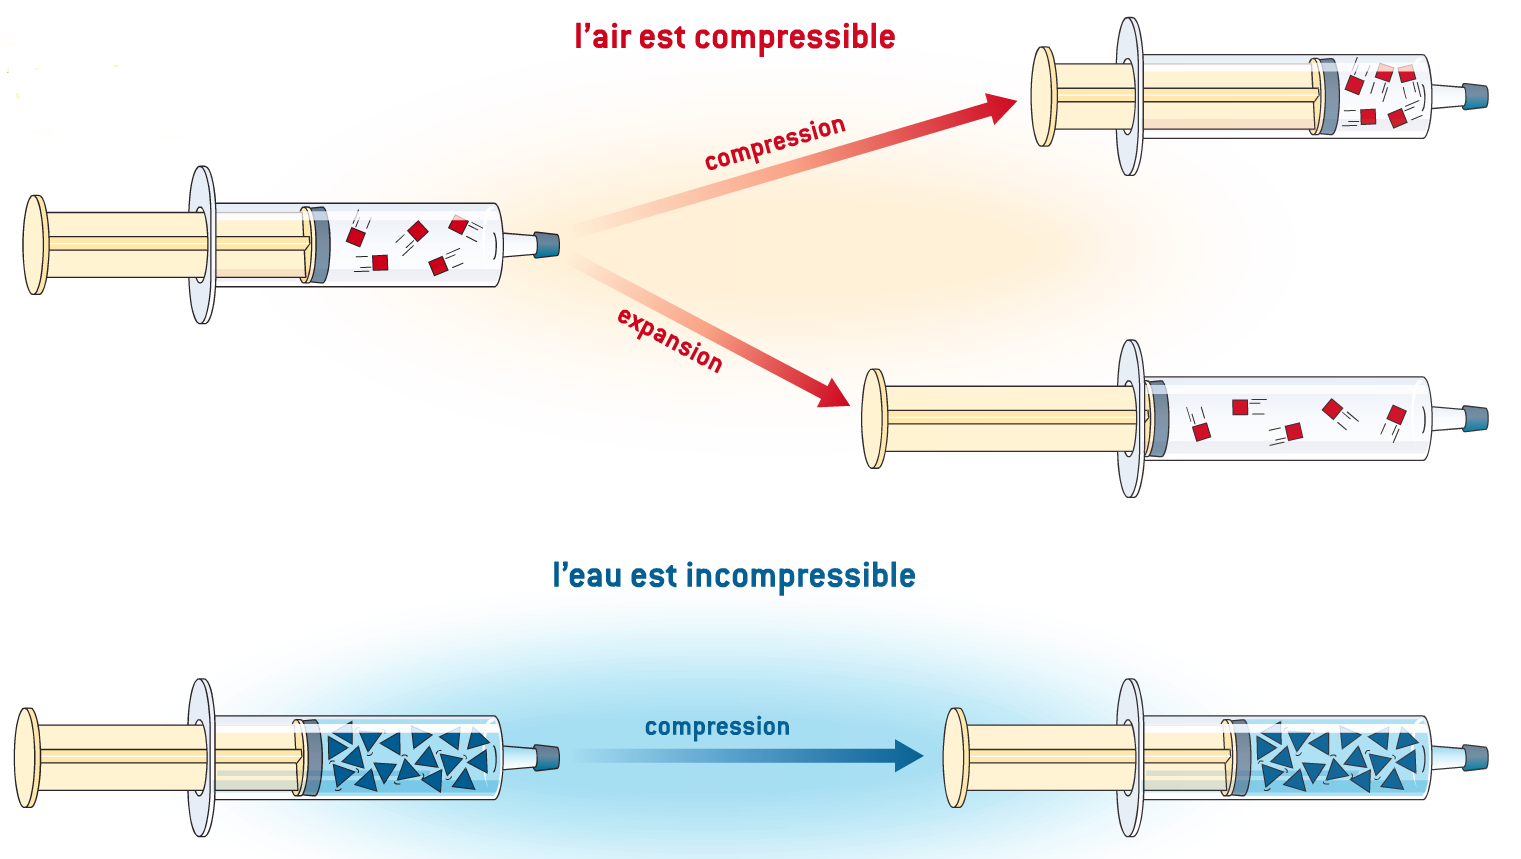
\includegraphics[scale=0.25]{../img/compression}
\end{center}
\end{frame}


\section{Pression d'un gaz}

\begin{frame}
\begin{mybilan}
	\begin{itemize}
		\item La \kw{pression} d'un gaz correspond aux chocs des grains de matières entre eux ou contre les parois.\pause
		\item Plus on compresse un gaz, plus les chocs sont nombreux et plus la pression augmente.\pause
		\item \kw{L'unité légale de pression} est le \kw{pascal (Pa)}.\pause
		\item Pour mesurer la pression d'un gaz on utilise un \kw{manomètre}.
		
	\end{itemize}
\end{mybilan}
\end{frame}
\section{Masse volumique de l'air}


\subsection{Masse de l'air}

\begin{frame}
\begin{mybilan}
	Dans des conditions normales de température et de pression, 1l d'air à une masse d'air est de \num{1.2} g.
\end{mybilan}
\end{frame}

\subsection{Masse volumique}

\begin{frame}
\begin{mybilan}
	La \kw{masse volumique} d'un corps, notée \kw{$\rho$}, est le rapport entre la masse \kw{m} et son volume \kw{V}. Elle est spécifique à chaque matière pour une température et une pression donnée.
	
	\begin{equation*}
	\mathbf{\rho} \: \mathit{{\small (kg/m^3)}} = \frac{\mathbf{m} \mathit{{\small (kg)}}}{\mathbf{V} \mathit{{\small (m^3)}}}
	\end{equation*}
\end{mybilan}\pause

\begin{myex}
	\begin{itemize}
		\item $\rho_{air}  = \num{1.3} \: kg/m^3$ à 0°C et une pression de \num{1013} hPa.
		\item $\rho_{air}  = \num{1.2} \: kg/m^3$ à 20°C et une pression de \num{1013} hPa.
	\end{itemize}
\end{myex}

\end{frame}
\end{document}